% !TeX program = xelatex
\documentclass[10pt,handout]{beamer}

\usetheme{metropolis}

%\usepackage{pgfplots}
%\usepgfplotslibrary{dateplot}
\usepackage{pgfopts}
\usepackage{amsmath}
\usepackage{structuralanalysis}
\usepackage{tikz}
\usepackage{tikz-3dplot}
\usepackage{chngcntr}
\usepackage{wasysym}
\usepackage{mathtools}
\usepackage{alphalph}
\usepackage{xcolor}

\newcommand{\highlight}[1]{%
	\colorbox{red!50}{$\displaystyle#1$}}

\setcounter{lecture}{3}
\counterwithin{equation}{lecture}
\makeatletter
\def\user@resume{resume}
\def\user@intermezzo{intermezzo}
%
\newcounter{previousequation}
\newcounter{lastsubequation}
\newcounter{savedparentequation}
\setcounter{savedparentequation}{1}
% 
\renewenvironment{subequations}[1][]{%
	\def\user@decides{#1}%
	\setcounter{previousequation}{\value{equation}}%
	\ifx\user@decides\user@resume 
	\setcounter{equation}{\value{savedparentequation}}%
	\else  
	\ifx\user@decides\user@intermezzo
	\refstepcounter{equation}%
	\else
	\setcounter{lastsubequation}{0}%
	\refstepcounter{equation}%
	\fi\fi
	\protected@edef\theHparentequation{%
		\@ifundefined {theHequation}\theequation \theHequation}%
	\protected@edef\theparentequation{\theequation}%
	\setcounter{parentequation}{\value{equation}}%
	\ifx\user@decides\user@resume 
	\setcounter{equation}{\value{lastsubequation}}%
	\else
	\setcounter{equation}{0}%
	\fi
	\def\theequation  {\theparentequation  \alph{equation}}%
	\def\theHequation {\theHparentequation \alph{equation}}%
	\ignorespaces
}{%
%  \arabic{equation};\arabic{savedparentequation};\arabic{lastsubequation}
\ifx\user@decides\user@resume
\setcounter{lastsubequation}{\value{equation}}%
\setcounter{equation}{\value{previousequation}}%
\else
\ifx\user@decides\user@intermezzo
\setcounter{equation}{\value{parentequation}}%
\else
\setcounter{lastsubequation}{\value{equation}}%
\setcounter{savedparentequation}{\value{parentequation}}%
\setcounter{equation}{\value{parentequation}}%
\fi\fi
%  \arabic{equation};\arabic{savedparentequation};\arabic{lastsubequation}
\ignorespacesafterend
}
\makeatother
\title{AE 737 - Mechanics of Damage Tolerance}
\subtitle{Lecture 3}
\date{26 January 2016}
\author{Dr. Nicholas Smith}
\institute{Wichita State University, Department of Aerospace Engineering}
% \titlegraphic{\hfill\includegraphics[height=1.5cm]{logo/logo}}

\begin{document}

\maketitle

\begin{frame}{office hours}
	\begin{itemize}
		\item Official office hours will be Fridays from 3:00 - 5:00
		\item Homeworks will generally be due on Tuesday
		\item I can make time to meet outside of office hours, just send an e-mail to make an appointment
	\end{itemize}
\end{frame}

\begin{frame}{schedule}
	\begin{itemize}
		\item 26 Jan - Superposition, Compounding
		\item 28 Jan - Plastic Zone, 
		\item 2 Feb - Plastic Zone, Homework 1 Due, Homework 2 Assigned
		\item 4 Feb - Plastic Zone
		\item 9 Feb - Fracture Toughness, Homework 2 Due
	\end{itemize}
\end{frame}

\begin{frame}
  \frametitle{outline}
  \setbeamertemplate{section in toc}[sections numbered]
  \tableofcontents[hideallsubsections]
\end{frame}

\section{review}

\begin{frame}{example 1}
	\begin{enumerate}
		\item 
		\begin{enumerate}
			\item Determine the value of $K_I$ for a center-cracked panel with $W/2a = 3$ and a uniformly applied remote stress, $\sigma$.
			\item Determine the value of $K_I$ for an edge-cracked panel with $W/a = 3$ and a uniformly applied remote stress, $\sigma$.
			\item Compare these two results. Note that in both cases the panel width to crack length ratio is the same.
		\end{enumerate}
	\end{enumerate}
\end{frame}

\begin{frame}{example 1}
	\begin{itemize}
		\item Comparing the two cases, we see that the finite width effects are much more significant for the edge-crack specimen
		\item The edge-crack specimen is also overall more effected by a crack of that relative length.
		\item Why are they not the same?
	\end{itemize}
\end{frame}

\begin{frame}{example 1}
	\begin{figure}
	\centering
	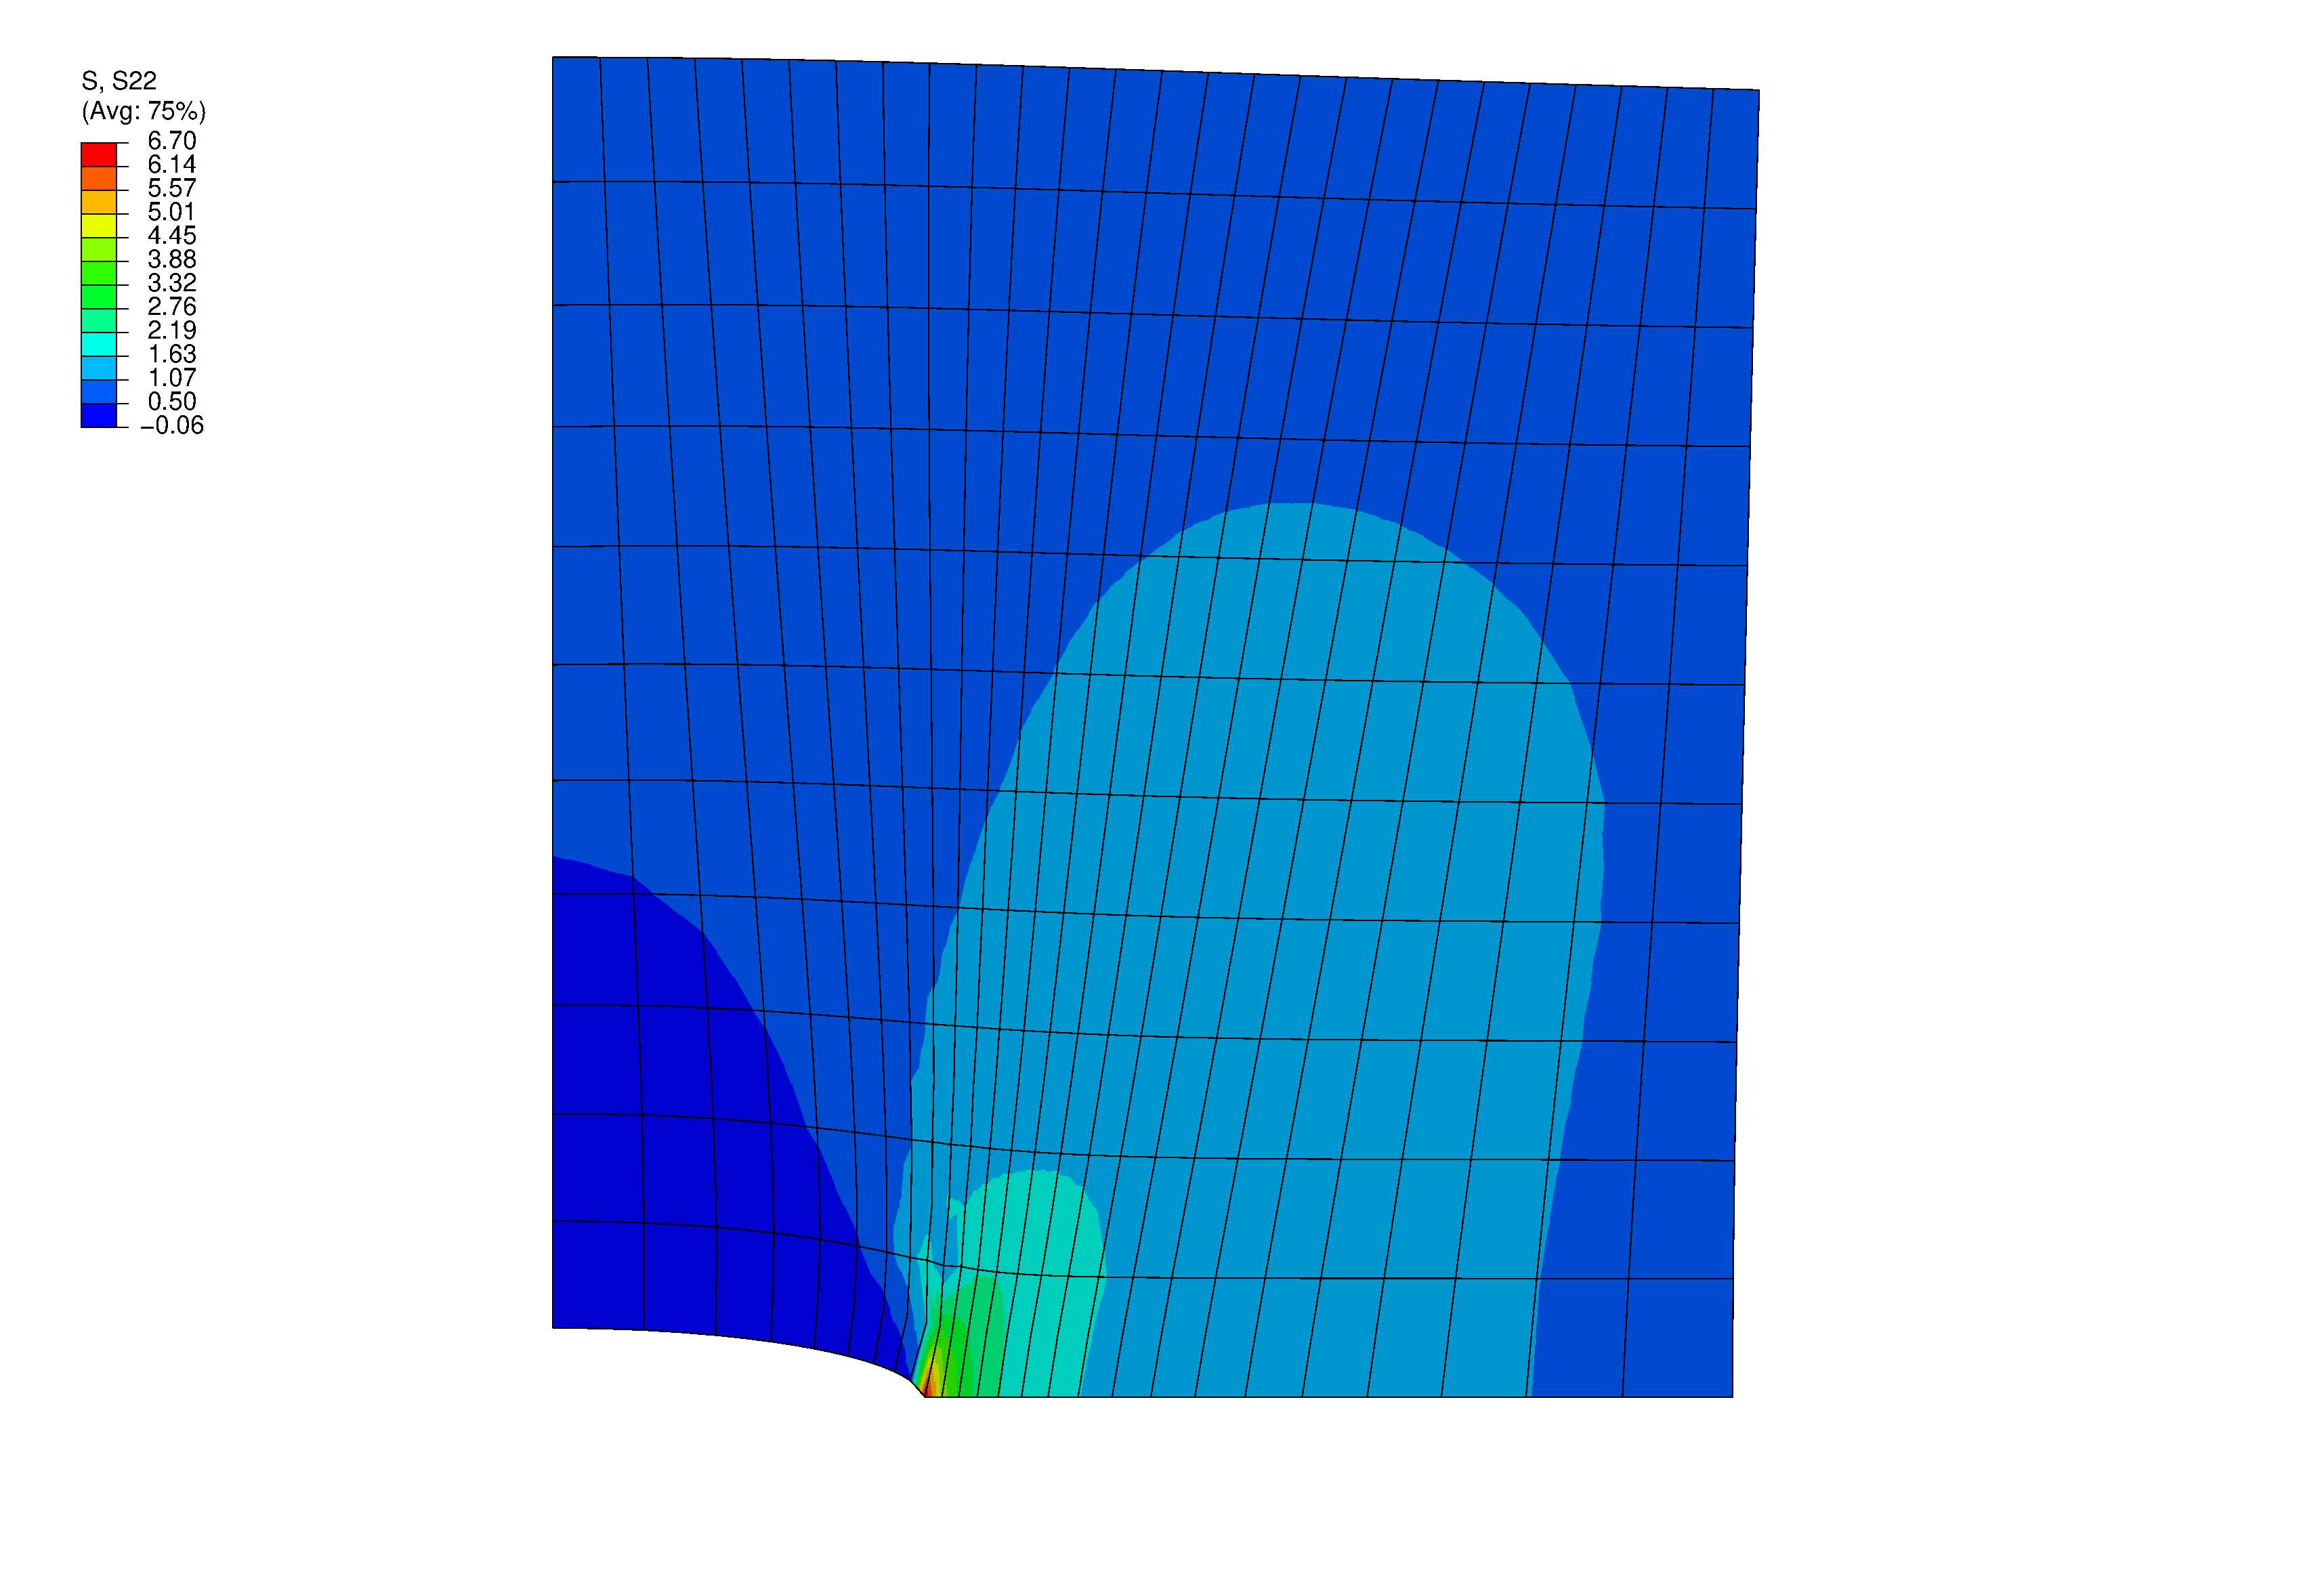
\includegraphics[width=0.9\linewidth]{center-crack}
	\caption{center-crack finite element simulation}
	\label{fig:center-crack}
	\end{figure}
\end{frame}

\begin{frame}{example 1}
	\begin{figure}
	\centering
	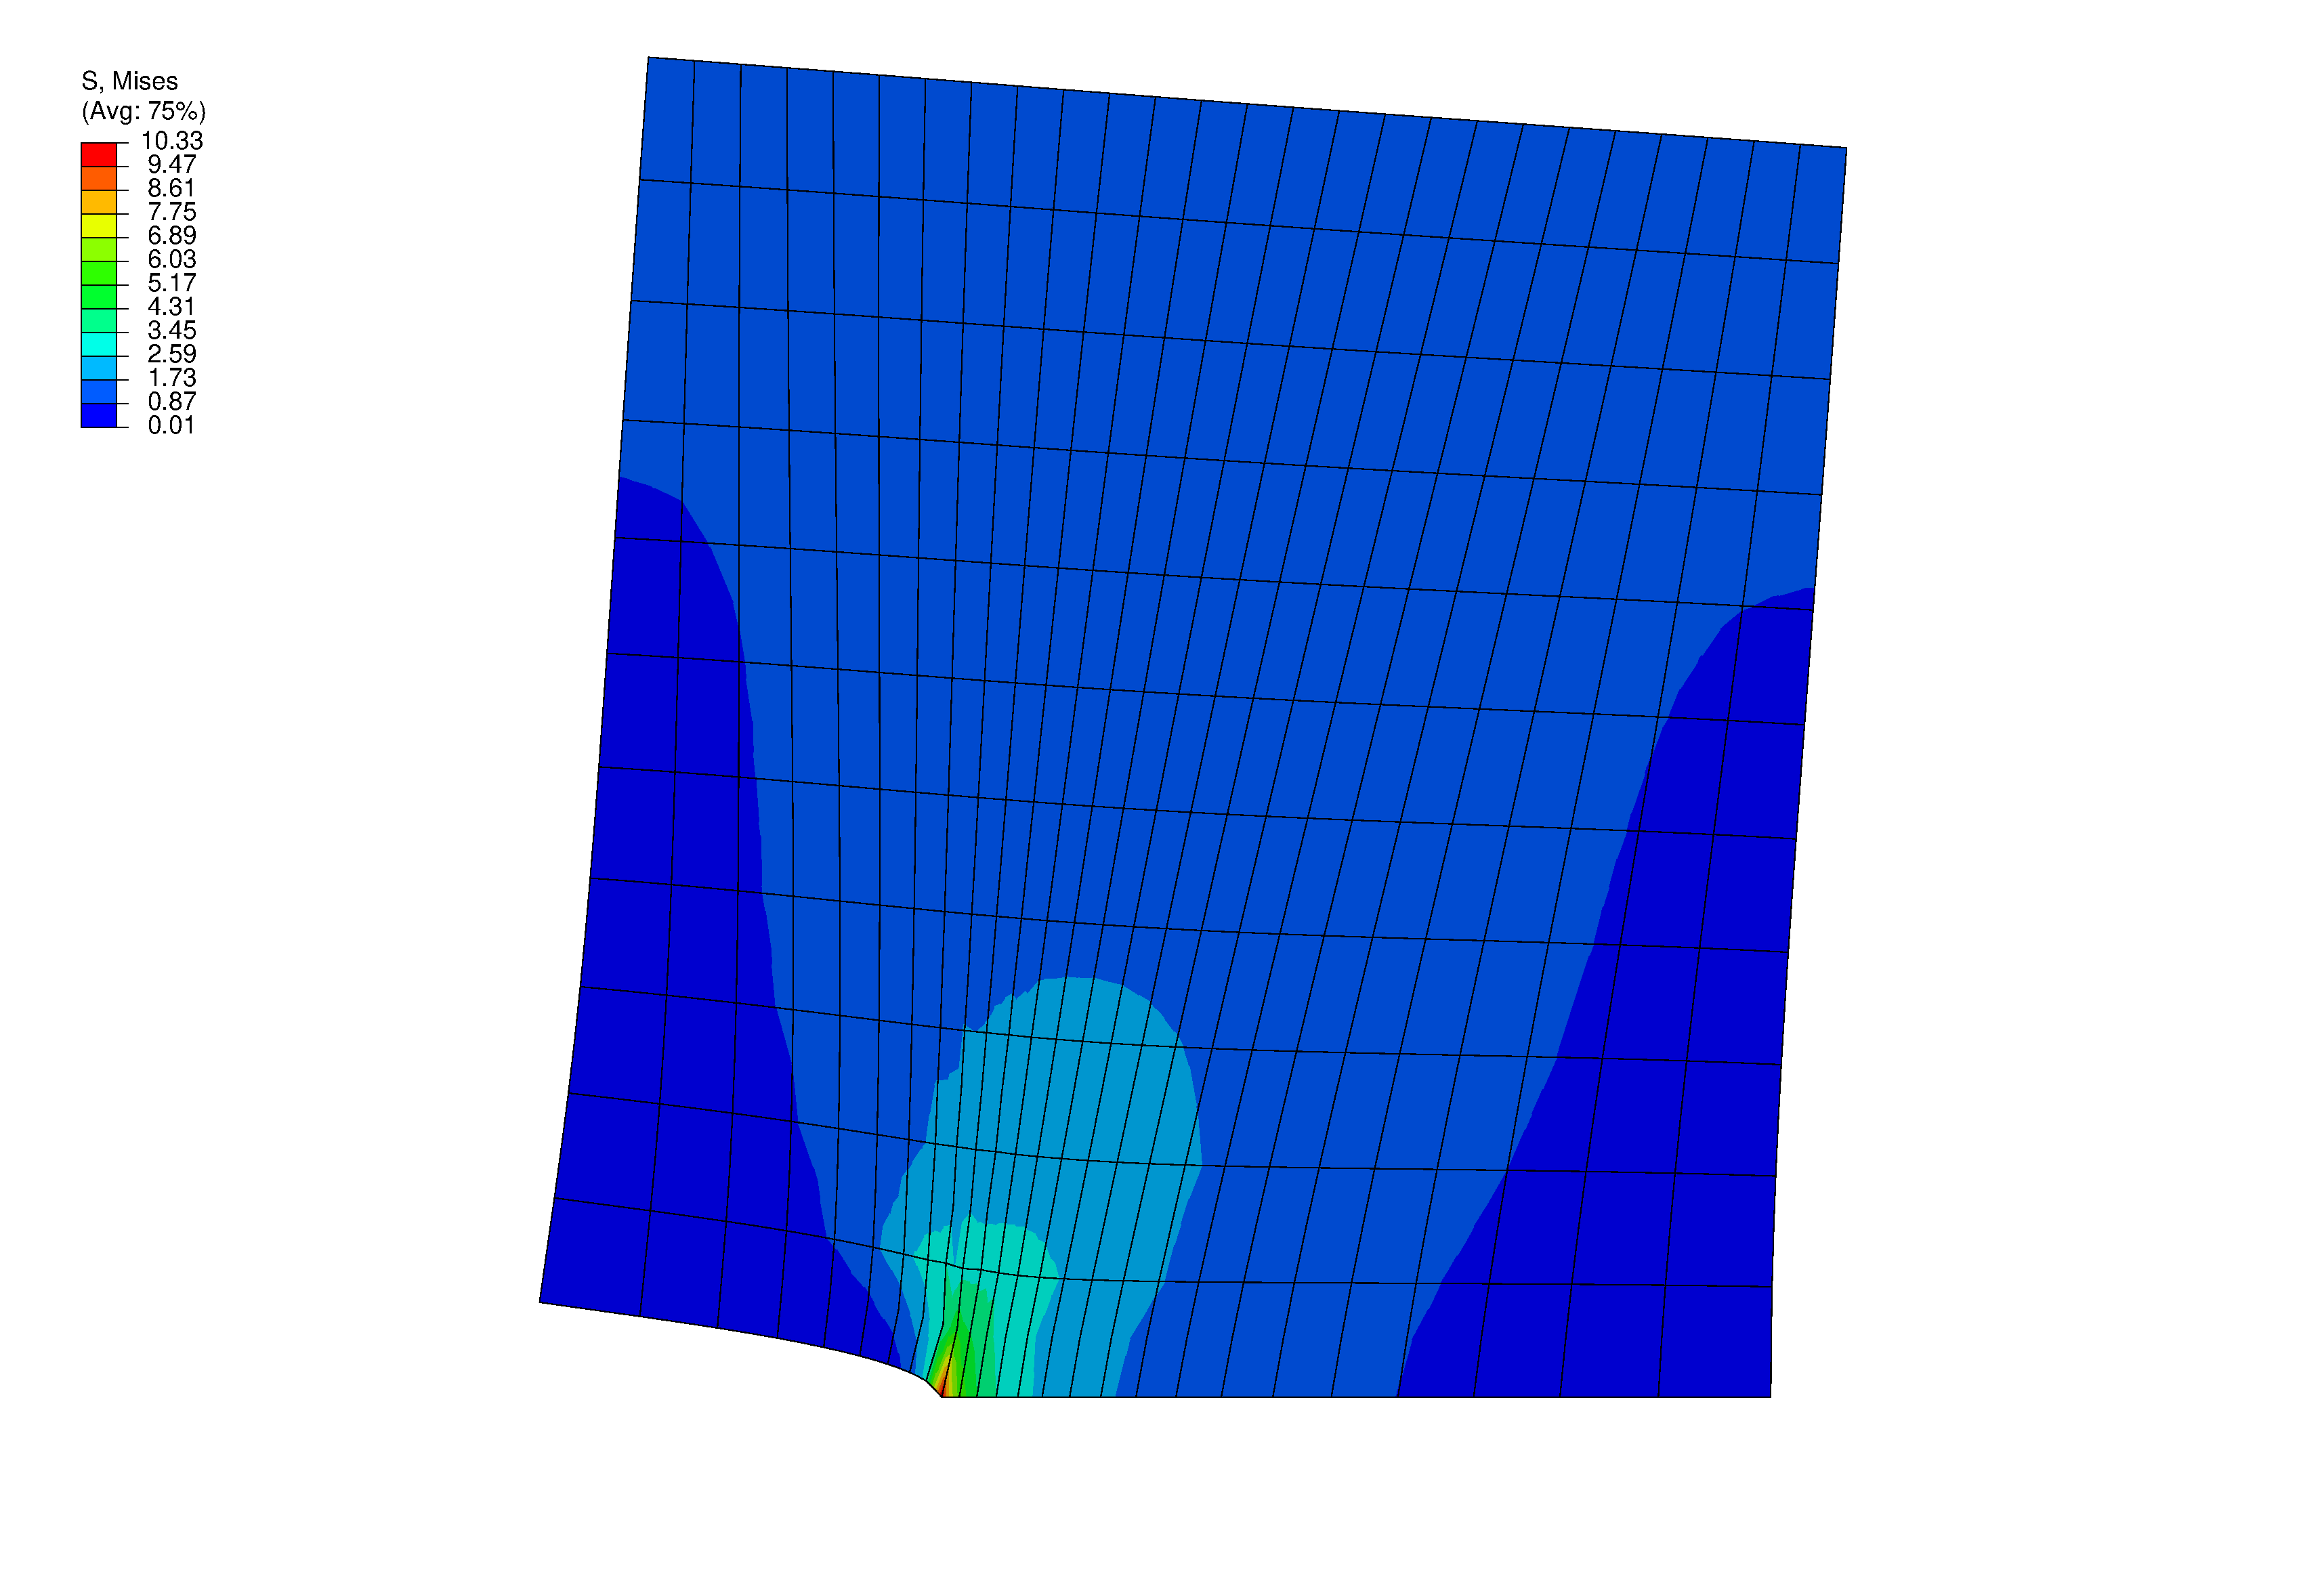
\includegraphics[width=0.9\linewidth]{edge-crack}
	\caption{edge-crack finite element simulation}
	\label{fig:edge-crack}
	\end{figure}
\end{frame}

\section{2D cracks at a hole}

\begin{frame}{when to consider 2D crack shape}
	\begin{itemize}
		\item When do we need to worry about 2D crack shape?
		\item The important factor is ratio of crack length to thickness
		\item When crack length is less than 5 times thickness, 2D shape effects are not negligible
	\end{itemize}
\end{frame}

\begin{frame}{cracks around a hole}
	\begin{figure}
		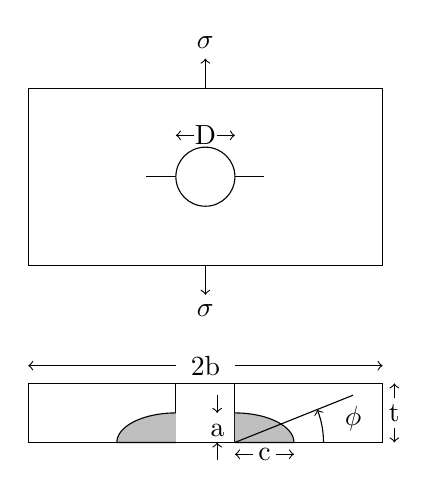
\begin{tikzpicture}
		\begin{scope}[scale=.75]
		\draw (0,-1.5) -- (0,1.5) -- (6,1.5) -- (6,-1.5) -- (0,-1.5);
		\draw[->] (3,1.5) -- (3,2) node[above] {$\sigma$};
		\draw[->] (3,-1.5) -- (3,-2) node[below] {$\sigma$};
		\draw (3,0) circle (0.5);
		\draw (3.5,0) -- (4,0);
		\draw (2.5,0) -- (2,0);
		\draw node at (3,-3.2) {2b};
		\draw[->] (2.5,-3.2) -- (0,-3.2);
		\draw[->] (3.5,-3.2) -- (6,-3.2);
		\draw node at (3,0.7) {D};
		\draw[->] (3.2,0.7) -- (3.5,0.7);
		\draw[->] (2.8,0.7) -- (2.5,0.7);
		\draw (0,-3.5) -- (6,-3.5) -- (6,-4.5) -- (0,-4.5) -- (0,-3.5);
		\draw (3.5,-3.5) -- (3.5,-4.5);
		\draw (2.5,-3.5) -- (2.5,-4.5);
		\draw node at (6.2,-4) {t};
		\draw node at (3.2,-4.3) {a};
		\draw node at (4,-4.7) {c};
		\draw[->] (6.2,-3.75) -- (6.2,-3.5);
		\draw[->] (6.2,-4.25) -- (6.2,-4.5);
		\draw[fill=gray!50] (3.5,-4) arc (90:0:1.0 and 0.5) -- (3.5,-4.5);
		\draw[fill=gray!50] (2.5,-4) arc (90:180:1.0 and 0.5) -- (2.5,-4.5);
		\draw[->] (4.2,-4.7) -- (4.5,-4.7);
		\draw[->] (3.8,-4.7) -- (3.5,-4.7);
		\draw[->] (3.2,-4.8) -- (3.2,-4.5);
		\draw[->] (3.2,-3.7) -- (3.2,-4.0);
		\draw (3.5,-4.5) -- (5.5,-3.7);
		\draw[->] (5,-4.5) arc (0:21.8:1.5);
		\draw node at (5.5,-4.1) {$\phi$};
		\end{scope}
		\end{tikzpicture}
	\end{figure}
\end{frame}

\begin{frame}{remote stress}
	\begin{subequations}
		\begin{align}
		K_{I} &= \sigma \sqrt{\pi a} \beta\\
		\beta &= \sqrt{\frac{1}{Q}} F_{ch}\\
		F_{ch} &= \left(M_1 + M_2 \left(\frac{a}{t}\right)^2 + M_3 \left(\frac{a}{t}\right)^4\right)g_1 g_2 g_3 g_4 f_\phi f_w\\
		f_w &= \sqrt{\sec \left(\frac{\pi r}{2b}\right)\sec \left(\frac{\pi (2r + nc)}{4(b-c) + 2nc} \sqrt{\frac{a}{t}}\right)}\\
		g_2 &= \frac{1+0.358\lambda+1.425\lambda^2 - 1.578\lambda^3+2.156\lambda^4}{1+0.13\lambda^2}\\
		\lambda &= \frac{1}{1+(c/r)\cos \left(0.85 \phi \right)}
		\end{align}
		Where $n = $ number of cracks (1 or 2)
	\end{subequations}
\end{frame}

\begin{frame}{remote stress}
	For $a/c \le 1$
	\begin{subequations}[resume]
		\begin{align}
		M_1 &= 1.13 - 0.09 \left(\frac{a}{c}\right)\\
		M_2 &= -0.54 + \frac{0.89}{0.2 + \frac{a}{c}}\\
		M_3 &= 0.5 - \frac{1}{0.65 + \frac{a}{c}}+ 14 \left(1-\frac{a}{c}\right)^{24}\\
		Q &= 1+1.464\left(\frac{a}{c}\right)^{1.65}\\
		g_1 &= 1 + \left(0.1+0.35 \left(a/t\right)^2\right)(1-\sin \phi)^2\\
		g_3 &= (1+0.04 (a/c))\left(1+0.1(1-\cos \phi)^2\right)\left(0.85+0.15(a/t)^{1/4}\right)\\
		g_4 &= 1 - 0.7(1-a/t)(a/c-0.2)(1-a/c)\\
		f_\phi &= \left(\left(\frac{a}{c}\right)^2 \cos^2 \phi + \sin^2 \phi \right)^{1/4}
		\end{align}
	\end{subequations}
\end{frame}

\begin{frame}{remote stress}
	For $a/c > 1$
	\begin{subequations}[resume]
		\begin{align}
		M_1 &= \sqrt{c/a}(1+0.04 (c/a))\\
		M_2 &= 0.2(c/a)^4\\
		M_3 &= -0.11(c/a)^4\\
		Q &= 1+1.464\left(\frac{c}{a}\right)^{1.65}\\
		g_1 &= 1 + \left(0.1+0.35 (c/a)\left(a/t\right)^2\right)(1-\sin \phi)^2\\
		g_3 &= (1.13-0.09 (c/a))\left(1+0.1(1-\cos \phi)^2\right)\left(0.85+0.15(a/t)^{1/4}\right)\\
		g_4 &= 1 \\
		f_\phi &= \left(\cos^2 \phi + \left(\frac{c}{a}\right)^2 \sin^2 \phi \right)^{1/4}
		\end{align}
	\end{subequations}
\end{frame}

\begin{frame}{remote stress}
	\begin{itemize}
		\item The same formulas apply for both symmetric cracks ($n=2$) and a single crack ($n=1$) with one additional correction factor applied to the single crack case
		\begin{equation}
		K_{I,single} = \sqrt{\frac{4/\pi + ac/2tr}{4/\pi + ac/tr}}K_{I,symmetric}
		\end{equation}
	\end{itemize}
\end{frame}

\begin{frame}{surface cracks around a hole}
	\begin{figure}
		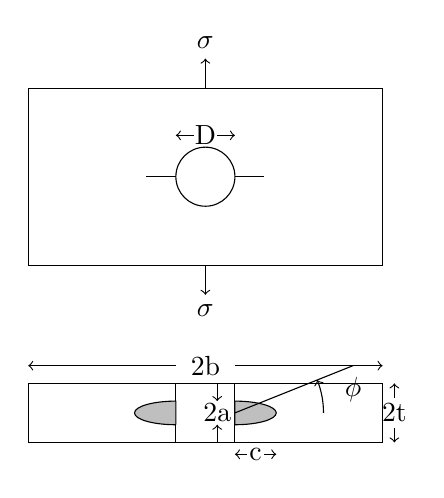
\begin{tikzpicture}
		\begin{scope}[scale=.75]
		\draw (0,-1.5) -- (0,1.5) -- (6,1.5) -- (6,-1.5) -- (0,-1.5);
		\draw[->] (3,1.5) -- (3,2) node[above] {$\sigma$};
		\draw[->] (3,-1.5) -- (3,-2) node[below] {$\sigma$};
		\draw (3,0) circle (0.5);
		\draw (3.5,0) -- (4,0);
		\draw (2.5,0) -- (2,0);
		\draw node at (3,-3.2) {2b};
		\draw[->] (2.5,-3.2) -- (0,-3.2);
		\draw[->] (3.5,-3.2) -- (6,-3.2);
		\draw node at (3,0.7) {D};
		\draw[->] (3.2,0.7) -- (3.5,0.7);
		\draw[->] (2.8,0.7) -- (2.5,0.7);
		\draw (0,-3.5) -- (6,-3.5) -- (6,-4.5) -- (0,-4.5) -- (0,-3.5);
		\draw (3.5,-3.5) -- (3.5,-4.5);
		\draw (2.5,-3.5) -- (2.5,-4.5);
		\draw node at (6.2,-4) {2t};
		\draw node at (3.2,-4) {2a};
		\draw node at (3.85,-4.7) {c};
		\draw[->] (6.2,-3.75) -- (6.2,-3.5);
		\draw[->] (6.2,-4.25) -- (6.2,-4.5);
		\draw[fill=gray!50] (3.5,-4.2) arc (-90:90:0.7 and 0.2) -- (3.5,-4.2);
		\draw[fill=gray!50] (2.5,-4.2) arc (270:90:0.7 and 0.2) -- (2.5,-4.2);
		\draw[->] (4,-4.7) -- (4.2,-4.7);
		\draw[->] (3.7,-4.7) -- (3.5,-4.7);
		\draw[->] (3.2,-4.5) -- (3.2,-4.2);
		\draw[->] (3.2,-3.5) -- (3.2,-3.8);
		\draw (3.5,-4.0) -- (5.5,-3.2);
		\draw[->] (5,-4.) arc (0:21.8:1.5);
		\draw node at (5.5,-3.6) {$\phi$};
		\end{scope}
		\end{tikzpicture}
	\end{figure}
\end{frame}

\begin{frame}{remote stress}
	\begin{subequations}
		\begin{align}
		K_{I} &= \sigma \sqrt{\pi a} \beta\\
		\beta &= \sqrt{\frac{1}{Q}} F_{sh}\\
		F_{sh} &= \left(M_1 + M_2 \left(\frac{a}{t}\right)^2 + M_3 \left(\frac{a}{t}\right)^4\right)g_1 g_2 g_3 f_\phi f_w\\
		f_w &= \sqrt{\sec \left(\frac{\pi r}{2b}\right)\sec \left(\frac{\pi (2r + nc)}{4(b-c) + 2nc} \sqrt{\frac{a}{t}}\right)}\\
		M_2 &= \frac{0.05}{0.11 + (a/c)^{3/2}}\\
		M_3 &= \frac{0.29}{0.23 + (a/c)^{3/2}}
		\end{align}
		Where $n = $ number of cracks (1 or 2)
	\end{subequations}
\end{frame}

\begin{frame}{remote stress}
	\begin{subequations}[resume]
		\begin{align}
		g_1 &= 1- \frac{(a/t)^4(2.6-2a/t)^{1/2}}{1+4a/c}\cos \phi\\
		g_2 &= \frac{1+0.358\lambda+1.425\lambda^2 - 1.578\lambda^3+2.156\lambda^4}{1+0.08\lambda^2}\\
		\lambda &= \frac{1}{1+(c/r)\cos \left(0.9 \phi \right)}\\
		g_3 &= 1+0.1(1-\cos \phi)^2 (1-a/t)^{10}
		\end{align}
	\end{subequations}
\end{frame}

\begin{frame}{remote stress}
	If $a/c \le 1$
	\begin{subequations}[resume]
		\begin{align}
		Q &= 1 + 1.464(a/c)^{1.65}\\
		M_1 &= 1\\
		f_\phi &= \left(\left(\frac{a}{c}\right)^2 \cos^2 \phi + \sin^2 \phi \right)^{1/4}
		\end{align}
	If $a/c > 1$
		\begin{align}
		Q &= 1 + 1.464(c/a)^{1.65}\\
		M_1 &= \sqrt{c/a}\\
		f_\phi &= \left(\cos^2 \phi + \left(\frac{c}{a}\right)^2 \sin^2 \phi \right)^{1/4}
		\end{align}
	\end{subequations}
\end{frame}

\begin{frame}{single-crack correction}
	\begin{itemize}
		\item When the surface crack is only on one side of the hole, we use the same correction as for corner cracks
		\begin{equation}
		K_{I,single} = \sqrt{\frac{4/\pi + ac/2tr}{4/\pi + ac/tr}}K_{I,symmetric}
		\end{equation}
	\end{itemize}
\end{frame}

\begin{frame}{edge crack on a lug}
	\begin{figure}
		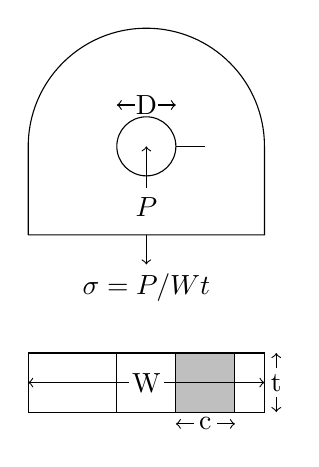
\begin{tikzpicture}
		\begin{scope}[scale=.75]
		\draw (1,-1.5) -- (1,0) arc (180:0:2) -- (5,-1.5) -- (1,-1.5);
		\draw[->] (3,-1.5) -- (3,-2) node[below] {$\sigma = P/Wt$};
		\draw (3,0) circle (0.5);
		\draw (3.5,0) -- (4,0);
		\draw node at (3,-4) {W};
		\draw node at (3,0.7) {D};
		\draw[->] (3,-0.7) node[below]{$P$} -- (3,0);
		\draw[->] (3.2,0.7) -- (3.5,0.7);
		\draw[->] (2.8,0.7) -- (2.5,0.7);
		\draw (1,-3.5) -- (5,-3.5) -- (5,-4.5) -- (1,-4.5) -- (1,-3.5);
		\draw (3.5,-3.5) -- (3.5,-4.5);
		\draw (2.5,-3.5) -- (2.5,-4.5);
		\draw node at (5.2,-4) {t};
		\draw node at (4,-4.7) {c};
		\draw[->] (5.2,-3.75) -- (5.2,-3.5);
		\draw[->] (5.2,-4.25) -- (5.2,-4.5);
		\draw[fill=gray!50] (3.5,-3.5) -- (4.5,-3.5) -- (4.5,-4.5) -- (3.5,-4.5);
		\draw[->] (4.2,-4.7) -- (4.5,-4.7);
		\draw[->] (3.8,-4.7) -- (3.5,-4.7);
		\draw[->] (2.7,-4) -- (1,-4);
		\draw[->] (3.3,-4) -- (5,-4);
		\end{scope}
		\end{tikzpicture}
	\end{figure}
\end{frame}

\begin{frame}{edge crack on a lug}
	\begin{subequations}
		\begin{align}
		K_I &= \sigma_{br} \sqrt{\pi c} \beta\\
		\beta &= \left(\frac{G_0 D}{2W} + G_1\right)G_w G_L G_2\\
		z &= \left(1+\frac{2C}{D}\right)^{-1}\\
		G_0 &= 0.7071 + 0.7548z + 0.3415z^2 + 0.642z^3 + 0.9196z^4\\
		G_1 &= 0.078z + 0.7588z^2 - 0.4293z^3 + 0.0644z^4 + 0.651z^5\\
		G_L &= \left(\sec \left(\frac{\pi D}{2W}\right)\right)^{1/2}\\
		\lambda &= \frac{\pi}{2} \left(\frac{D+c}{W-c}\right)\\
		G_w &= \left(\sec \lambda \right)^{1/2}
		\end{align}
	\end{subequations}
\end{frame}

\begin{frame}{edge crack on a lug}
	\begin{subequations}[resume]
		\begin{align}
		b &= \frac{W-D}{2}\\
		A_1 &= 0.688 + 0.772 \frac{D}{W} + 0.613 \left(\frac{D}{W}\right)^2\\
		A_2 &= 4.948 - 17.318 \frac{D}{W} + 16.785 \left(\frac{D}{W}\right)^2\\
		A_3 &= -14.297 + 62.994 \frac{D}{W} - 69.818 \left(\frac{D}{W}\right)^2\\
		A_4 &= 12.35 - 58.644 \frac{D}{W} + 66.387 \left(\frac{D}{W}\right)^2\\
		G_2 &= A_1 + A_2 \frac{c}{b} + A_3 \left(\frac{c}{b}\right)^2 + A_4 \left(\frac{c}{b}\right)^3
		\end{align}
	\end{subequations}
\end{frame}

\begin{frame}{corner crack on a lug}
	\begin{figure}
		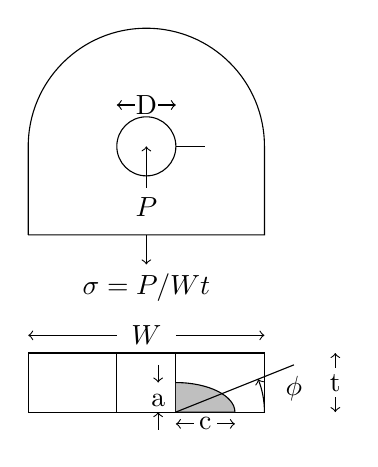
\begin{tikzpicture}
		\begin{scope}[scale=.75]
		\draw (1,-1.5) -- (1,0) arc (180:0:2) -- (5,-1.5) -- (1,-1.5);
		\draw[->] (3,-1.5) -- (3,-2) node[below] {$\sigma = P/Wt$};
		\draw (3,0) circle (0.5);
		\draw (3.5,0) -- (4,0);
		\draw node at (3,0.7) {D};
		\draw[->] (3,-0.7) node[below]{$P$} -- (3,0);
		\draw[->] (3.2,0.7) -- (3.5,0.7);
		\draw[->] (2.8,0.7) -- (2.5,0.7);
		\draw (1,-3.5) -- (5,-3.5) -- (5,-4.5) -- (1,-4.5) -- (1,-3.5);
		\draw (3.5,-3.5) -- (3.5,-4.5);
		\draw (2.5,-3.5) -- (2.5,-4.5);
		\draw node at (6.2,-4) {t};
		\draw node at (3.2,-4.3) {a};
		\draw node at (4,-4.7) {c};
		\draw[->] (6.2,-3.75) -- (6.2,-3.5);
		\draw[->] (6.2,-4.25) -- (6.2,-4.5);
		\draw[fill=gray!50] (3.5,-4) arc (90:0:1.0 and 0.5) -- (3.5,-4.5);
		\draw[->] (4.2,-4.7) -- (4.5,-4.7);
		\draw[->] (3.8,-4.7) -- (3.5,-4.7);
		\draw[->] (3.2,-4.8) -- (3.2,-4.5);
		\draw[->] (3.2,-3.7) -- (3.2,-4.0);
		\draw (3.5,-4.5) -- (5.5,-3.7);
		\draw[->] (5,-4.5) arc (0:21.8:1.5);
		\draw node at (5.5,-4.1) {$\phi$};
		\draw node at (3,-3.2) {$W$};
		\draw[->] (2.5,-3.2) -- (1,-3.2);
		\draw[->] (3.5,-3.2) -- (5,-3.2);
		\end{scope}
		\end{tikzpicture}
	\end{figure}
\end{frame}

\begin{frame}{corner crack on a lug}
	\begin{subequations}
		\begin{align}
		\beta &= \left(\frac{G_0 D}{2W} + G_1\right)G_w\\
		z &= \left(1 + 2\frac{c}{D} \cos (0.85 \phi)\right)^{-1}\\
		f_0(z) &= 0.7071 + 0.7548z + 0.3415z^2 + 0.642z^3 + 0.9196z^4\\
		f_1(z) &= 0.078z + 0.7588z^2 - 0.4293z^3 + 0.0644z^4 + 0.651z^5\\
		G_0 &= \frac{f_0(z)}{d_0}\\
		d_0 &= 1 + 0.13z^2\\
		g_p &= \left(\frac{W+D}{W-D}\right)^{1/2}\\
		G_1 &= f_1(z) \left(\frac{g_p}{d_0}\right)
		\end{align}
	\end{subequations}
\end{frame}

\begin{frame}{corner crack on a lug}
	\begin{subequations}[resume]
		\begin{align}
		G_w &= M_0 g_1 g_3 g_4 f_\phi f_w f_x\\
		v &= \frac{a}{t}\\
		\lambda &= \frac{pi}{2} \sqrt{v} \left(\frac{D+c}{W-c}\right)\\
		f_w &= \left(\sec \lambda \sec \frac{\pi D}{2W}\right)^{1/2}\\
		x &= \frac{a}{c}
		\end{align}
	\end{subequations}
\end{frame}

\begin{frame}{corner crack on a lug}
	For $a/c \le 1$
	\begin{subequations}[resume]
		\begin{align}
		f_\phi &= \left(\left(\frac{a}{c}\cos \phi\right)^2 + \sin^2 \phi \right)^{1/4}\\
		f_x &= \left(1+1.464 \left(\frac{a}{c}\right)^{1.65}\right)^{-1/2}\\
		&\begin{aligned}
		\mathllap{M_0} &= (1.13 - 0.09x) + \left(-0.54 + \frac{0.89}{0.2 + x}\right)v^2 \highlight{+} \\
		&\qquad \left(0.5 - \frac{1}{.65-x} + 14(1-x^{24})\right)v^4
		\end{aligned}\\
		g_1 &= 1 + \left(0.1 + 0.35 v^2\right)\left(1-\sin \phi\right)^2\\
		g_3 &= \left(1+0.04x\right)\left(1 + 0.1 \left(1-\cos \phi \right)^2\right)\left(0.85 + 0.15v ^{1/4}\right)\\
		g_4 &= 1 - 0.7 \left(1-v\right)\left(x - 0.2\right)\left(1-x\right)
		\end{align}
	\end{subequations}
\end{frame}

\begin{frame}{corner crack on a lug}
	For $a/c > 1$
	\begin{subequations}[resume]
		\begin{align}
		f_\phi &= \left(\left(\frac{ac}{c} \sin \phi \right)^2 + \cos^2 \phi \right)^{1/4}\\
		f_x &= \left(1 + 1.464 \left(\frac{c}{a}\right)^{1.65}\right)^{-1/2}\\
		M_0 &= x^{-1/2} + 0.04 x^{-3/2} + 0.2 x^{-4} v^2  - 0.11 x^{-4}v^4\\
		g_1 &= 1 + \left(0.1 + \frac{0.35}{x}v^2\right)\left(1-\sin \phi \right)^2\\
		g_3 &= \left(1.13 + \frac{0.09}{x}\right)\left(1+0.1(1-\cos \phi)^2\right)\left(0.85 + 0.15v^{1/4}\right)\\
		g_4 &= 1
		\end{align}
	\end{subequations}
\end{frame}

\begin{frame}{symmetric corner cracks under bending}
	\begin{figure}
		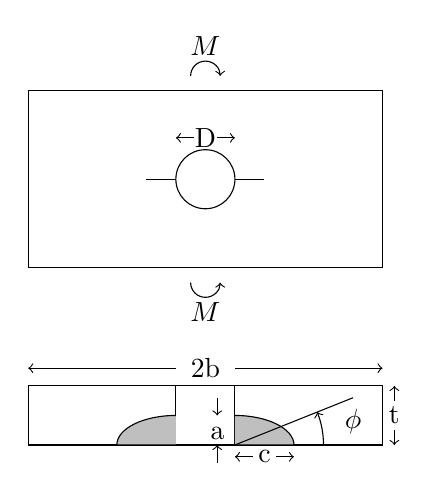
\begin{tikzpicture}
		\begin{scope}[scale=.75]
		\draw (0,-1.5) -- (0,1.5) -- (6,1.5) -- (6,-1.5) -- (0,-1.5);
		\draw[->] (2.75,1.75) arc (180:0:.25) node at (3,2.25) {$M$};
		\draw[->] (2.75,-1.75) arc (180:360:.25) node at (3,-2.25) {$M$};
		\draw (3,0) circle (0.5);
		\draw (3.5,0) -- (4,0);
		\draw (2.5,0) -- (2,0);
		\draw node at (3,-3.2) {2b};
		\draw[->] (2.5,-3.2) -- (0,-3.2);
		\draw[->] (3.5,-3.2) -- (6,-3.2);
		\draw node at (3,0.7) {D};
		\draw[->] (3.2,0.7) -- (3.5,0.7);
		\draw[->] (2.8,0.7) -- (2.5,0.7);
		\draw (0,-3.5) -- (6,-3.5) -- (6,-4.5) -- (0,-4.5) -- (0,-3.5);
		\draw (3.5,-3.5) -- (3.5,-4.5);
		\draw (2.5,-3.5) -- (2.5,-4.5);
		\draw node at (6.2,-4) {t};
		\draw node at (3.2,-4.3) {a};
		\draw node at (4,-4.7) {c};
		\draw[->] (6.2,-3.75) -- (6.2,-3.5);
		\draw[->] (6.2,-4.25) -- (6.2,-4.5);
		\draw[fill=gray!50] (3.5,-4) arc (90:0:1.0 and 0.5) -- (3.5,-4.5);
		\draw[fill=gray!50] (2.5,-4) arc (90:180:1.0 and 0.5) -- (2.5,-4.5);
		\draw[->] (4.2,-4.7) -- (4.5,-4.7);
		\draw[->] (3.8,-4.7) -- (3.5,-4.7);
		\draw[->] (3.2,-4.8) -- (3.2,-4.5);
		\draw[->] (3.2,-3.7) -- (3.2,-4.0);
		\draw (3.5,-4.5) -- (5.5,-3.7);
		\draw[->] (5,-4.5) arc (0:21.8:1.5);
		\draw node at (5.5,-4.1) {$\phi$};
		\end{scope}
		\end{tikzpicture}
	\end{figure}
\end{frame}

\begin{frame}{corner cracks under bending}
	\begin{subequations}
		\begin{align}
		\sigma_b &= \frac{Mt}{2 I}\\
		I &= \frac{bt^3}{6}\\
		\beta &= H_{ch} \left(\frac{a}{cQ}\right)^{1/2} F_{ch}\\
		H_{ch} &= H_1 + (H_2 - H_1) \sin ^p \phi\\
		H_1 &= 1 + G_{11} (a/t) + G_{12} (a/t)^2 + G_{13} (a/t)^3\\
		H_2 &= 1 + G_21 (a/t) + G_{22}(a/t)^2 + G_{23}(a/t)^3\\
		F_{ch} &= \left(M_1 + M_2(a/t)^2 + M_3(a/t)^4\right)g_1 g_2 g_3 g_4 f_\phi f_w\\
		\lambda &= \frac{1}{1 + (c/r) \cos (0.85 \phi)}\\
		g_2 &= \frac{1 + .358 \lambda + 1.425 \lambda^2 - 1.578 \lambda^3 + 2.156 \lambda^4}{1 + 0.13\lambda^2}
		\end{align}
	\end{subequations}
\end{frame}

\begin{frame}{corner cracks under bending}
	For $a/c \le 1$
	\begin{subequations}[resume]
		\begin{align}
		M_1 &= 1.13 - 0.09 (a/c)\\
		M_2 &= -0.54 + \frac{0.89}{0.2 + a/c}\\
		M_3 &= 0.5 - \frac{1}{0.65+a/c} + 14(1-a/c)^4\\
		Q &= 1 + 1.464(a/c)1.65\\
		g_1 &= 1 + \left(0.1 + (a/t) v^2\right)\left(1-\sin \phi\right)^2\\
		g_3 &= \left(1+0.04 (a/c) \right)\left(1 + 0.1 \left(1-\cos \phi \right)^2\right)\left(0.85 + 0.15(a/t) ^{1/4}\right)\\
		g_4 &= 1 - 0.7 \left(1-a/t\right)\left(a/c - 0.2\right)\left(1-a/c\right)
		\end{align}
	\end{subequations}
\end{frame}

\begin{frame}{corner cracks under bending}
	\begin{subequations}[resume]
		\begin{align}
		f_\phi &= \left(\left(\frac{a}{c}\cos \phi\right)^2 + \sin^2 \phi \right)^{1/4}\\
		G_{11} &= -0.43 - 0.74 a/c - 0.84 (a/c)^2\\
		G_{12} &= 1.25 - 1.19 a/c + 4.39 (a/c)^2\\
		G_{13} &= -1.94 + 4.22 a/c - 5.51 (a/c)^2\\
		G_{21} &= -1.5 - 0.04 a/c - 1.73 (a/c)^2\\
		G_{22} &= 1.71 - 3.17 a/c + 6.84 (a/c)^2\\
		G_{23} &= -1.28 + 2.71 a/c - 5.22 (a/c)^2\\
		p &= 0.1 + 1.3 a/t + 1.1 a/c - 0.7 (a/c) (a/t)
		\end{align}
	\end{subequations}
\end{frame}

\begin{frame}{corner cracks under bending}
	For $a/c > 1$
	\begin{subequations}[resume]
	\renewcommand{\theequation}{\theparentequation \alphalph{\value{equation}}}
		\begin{align}
		M_1 &= (c/a)^{1/2}(1+0.04 c/a)\\
		M_2 &= 0.2 (c/a)^4\\
		M_3 &= -0.11 (c/a)^4\\
		Q &= 1+ 1.464(c/a)^{1.65}\\
		g_1 &= 1 + \left(0.1 0.35(c/a)(a/t)^2\right)\left(1-\sin \phi\right)^2\\
		g_3 &= \left(1.13 - 0.09(c/a)\right)\left(1+ 0.1(1-\cos \phi)^2\right)\left(0.85 + 0.15(a/t)^{1/4}\right)\\
		g_4 &= 1
		\end{align}
	\end{subequations}
\end{frame}

\begin{frame}{corner cracks under bending}
	\begin{subequations}[resume]
	\renewcommand{\theequation}{\theparentequation \alphalph{\value{equation}}}
		\begin{align}
		f_\phi &= \left(\left(\cos^2 \phi + \frac{c}{a}\sin \phi\right)^2  \right)^{1/4}\\
		G_{11} &= -2.07 + 0.06 c/a\\
		G_{12} &= 4.35 + 0.16 c/a\\
		G_{13} &= -2.93 - 0.3c/a\\
		G_{21} &= -3.64 + 0.37c/a\\
		G_{22} &= 5.87 - 0.49c/a\\
		G_{23} &= -4.32 + 0.53c/a\\
		p &= 0.2 + c/a + 0.6a/t
		\end{align}
	\end{subequations}
\end{frame}

\begin{frame}{example 3}
	\begin{figure}[H]
		\centering
		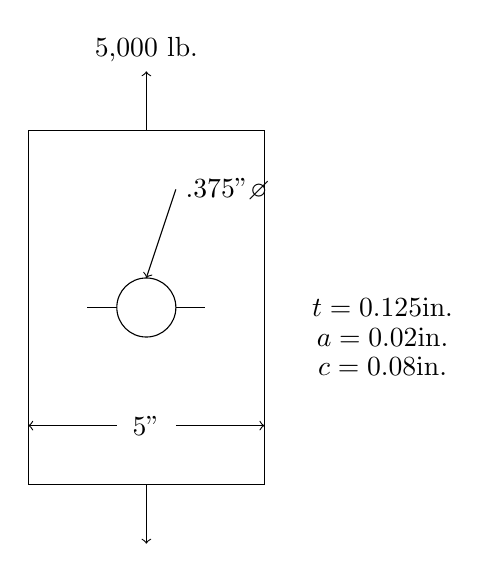
\begin{tikzpicture}
		\begin{scope}[scale=0.75]
		\draw (-2,3) -- (2,3) -- (2,-3) -- (-2,-3) -- (-2,3);
		\draw (0,0) circle (0.5cm);
		\draw (0.5,0) -- (1.0,0);
		\draw (-0.5,0) -- (-1.0,0);
		\draw[->] (0,3) -- (0,4) node[above] {5,000 lb.};
		\draw[->] (0,-3) -- (0,-4);
		\draw[->] (-0.5,-2) node at (0,-2) {5"} -- (-2,-2);
		\draw[->] (0.5,-2) -- (2,-2);
		\draw[->] (0.5,2) node[right] {.375"$\diameter$} -- (0,0.5); 
		\draw node at (4,0) {$t = 0.125 \text{in.}$};
		\draw node at (4,-0.5) {$a = 0.02 \text{in.}$};
		\draw node at (4,-1) {$c = 0.08 \text{in.}$};
		\end{scope}
		\end{tikzpicture}
		\label{fig:problem3}
	\end{figure}
\end{frame}

\begin{frame}{example 3}
	\begin{itemize}
		\item Case 1 - symmetric through cracks
		\item Case 2 - single through crack
		\item Case 3 - symmetric corner cracks
		\item Case 4 - single corner crack
		\item Case 5 - symmetric surface cracks
		\item Case 6 - single surface crack
	\end{itemize}
\end{frame}
\section{superposition}

\begin{frame}{superposition}
	\begin{itemize}
		\item Since the stress intensity factor is derived using Linear Elasticity, the principle of superposition applies
		\item Multiple applied loads can be superposed to find the effective stress intensity factor of the combined loading
	\end{itemize}
\end{frame}

\begin{frame}{superposition}
	\begin{figure}[H]
			\begin{tikzpicture}
			\point{a}{0}{1.5};
			\point{b}{3}{1.5};
			\point{c}{0}{-2};
			\point{d}{3}{-2};
			\draw (0,0) -- (0,1) -- (3,1) -- (3,-1) -- (0,-1) -- (0,0);
			\draw (1,0) -- (2,0);
			\draw node at (1.5,0.2) {2a};
			\lineload{3}{a}{b}[-.5][-.5];
			\draw node at (1.5,2) {$\sigma$};
			\lineload{3}{c}{d}[.5][.5];
			\draw node at (1.5,-2) {$\sigma$};
			\draw [->] (1.5,.5) -- (1.5,0.8) node[right] {$P$};
			\draw [->] (1.5,-.5) -- (1.5,-0.8) node[right] {$P$};
			\draw[fill=black] (1.5,.5) circle (0.03);
			\draw[fill=black] (1.5,-.5) circle (0.03);
			\draw[<->] (0.5,0) -- (0.5,0.5);
			\draw[<->] (0.5,0) -- (0.5,-0.5);
			\draw node at (0.3,0.25) {S} node at (0.3,-0.25) {S};
			\draw node at (3.5,0) {=};
			\point{e}{4}{1.5};
			\point{f}{7}{1.5};
			\point{g}{4}{-2};
			\point{h}{7}{-2};
			\draw (4,0) -- (4,1) -- (7,1) -- (7,-1) -- (4,-1) -- (4,0);
			\draw (5,0) -- (6,0);
			\draw node at (5.5,0.2) {2a};
			\lineload{3}{e}{f}[-.5][-.5];
			\draw node at (5.5,2) {$\sigma$};
			\lineload{3}{g}{h}[.5][.5];
			\draw node at (5.5,-2) {$\sigma$};
			\draw node at (7.5,0) {+};
			\draw (8,0) -- (8,1) -- (11,1) -- (11,-1) -- (8,-1) -- (8,0);
			\draw (9,0) -- (10,0);
			\draw node at (9.5,0.2) {2a};
			\draw [->] (9.5,.5) -- (9.5,0.8) node[right] {$P$};
			\draw [->] (9.5,-.5) -- (9.5,-0.8) node[right] {$P$};
			\draw[fill=black] (9.5,.5) circle (0.03);
			\draw[fill=black] (9.5,-.5) circle (0.03);
			\draw[<->] (8.5,0) -- (8.5,0.5);
			\draw[<->] (8.5,0) -- (8.5,-0.5);
			\draw node at (8.3,0.25) {S} node at (8.3,-0.25) {S};
			\end{tikzpicture}
		\end{figure}
\end{frame}

\begin{frame}{superposition}
	\begin{align*}
	K_I &= K_{I(\sigma)} + K_{I(P)}\\
	K_I &= \sigma\sqrt{\pi a} + \frac{P}{t\sqrt{\pi a}}\frac{1 - 0.5\left(\frac{a}{W}\right)+0.975\left(\frac{a}{W}\right)^2 - 0.16\left(\frac{a}{W}\right)^3}{\sqrt{1-\left(\frac{a}{W}\right)}}
	\end{align*}
\end{frame}

\begin{frame}{superposition}
	\begin{itemize}
		\item Sometimes, the superposition needed to solve a problem is not obvious
		\item It can be helpful to subtract a known solution from the problem
	\end{itemize}
\end{frame}

\begin{frame}{superposition}
	\begin{figure}[H]
		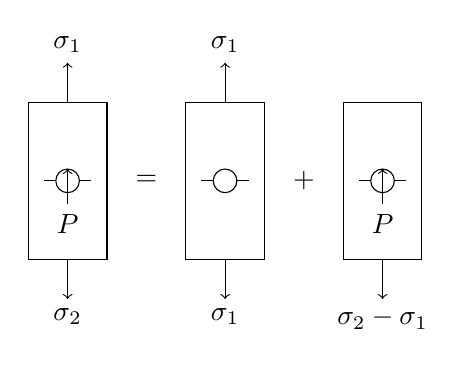
\begin{tikzpicture}
		\draw (0,-1) -- (0,1) -- (1,1) -- (1,-1) -- (0,-1);
		\draw[->] (0.5,1) -- (0.5,1.5) node[above] {$\sigma_1$};
		\draw[->] (0.5,-1) -- (0.5,-1.5) node[below] {$\sigma_2$};
		\draw (0.5,0) circle (0.15);
		\draw (0.35,0) -- (0.2,0);
		\draw (0.65,0) -- (0.8,0);
		\draw[->] (0.5,-0.3) node[below] {$P$} -- (0.5,0.15);
		\draw node at (1.5,0) {=};
		\draw (2,-1) -- (2,1) -- (3,1) -- (3,-1) -- (2,-1);
		\draw[->] (2.5,1) -- (2.5,1.5) node[above] {$\sigma_1$};
		\draw[->] (2.5,-1) -- (2.5,-1.5) node[below] {$\sigma_1$};
		\draw (2.5,0) circle (0.15);
		\draw (2.35,0) -- (2.2,0);
		\draw (2.65,0) -- (2.8,0);
		\draw node at (3.5,0) {+};
		\draw (4,-1) -- (4,1) -- (5,1) -- (5,-1) -- (4,-1);
		\draw[->] (4.5,-1) -- (4.5,-1.5) node[below] {$\sigma_2-\sigma_1$};
		\draw (4.5,0) circle (0.15);
		\draw (4.35,0) -- (4.2,0);
		\draw (4.65,0) -- (4.8,0);
		\draw[->] (4.5,-0.3) node[below] {$P$} -- (4.5,0.15);
		\end{tikzpicture}
	\end{figure}
\end{frame}

\section{compounding}

\begin{frame}{compounding}
	\begin{itemize}
		\item Different types of boundaries create different correction factors to the usual stress intensity factor
		\item We often use $\beta$ to indicate the total correction factor
		\item When multiple boundaries are present, we can combine them into one effective correction factor
		\item There are two general methods we use to create a compound correction factor
	\end{itemize}
\end{frame}

\begin{frame}{compounding method 1}
	\begin{itemize}
		\item The first method uses linear superposition, and thus is restricted to cases where the effect of each boundary can be assumed to add linearly
		\item While in most cases this is not strictly true, it provides a reasonable approximation
		\begin{equation}
		K_r = \bar{K} + \sum_{i=1}^{N}(K_i - \bar{K})
		\end{equation}
		\item Where $N$ is the number of boundaries, $\bar{K}$ is the stress intensity factor with no boundaries present and $K_i$ is the stress intensity factor associated with the $i^{\text{th}}$ boundary.
	\end{itemize}
\end{frame}

\begin{frame}{compounding method 1}
	\begin{itemize}
		\item We can rewrite this equation as
		\begin{equation}
		K_r = \sigma \sqrt{\pi a} \beta_r = \sigma \sqrt{\pi a} + \sum_{i=1}^{N}(\sigma \sqrt{\pi a}\beta_i - \sigma \sqrt{\pi a})
		\end{equation}
		\item Which leads to an expression for $\beta_r$ as
		\begin{equation}
		\beta_r = 1+\sum_{i=1}^{N} (\beta_i - 1)
		\end{equation}
	\end{itemize}
\end{frame}

\begin{frame}{compounding method 2}
	\begin{itemize}
		\item An alternative empirical method approximates the boundary effect as
		\begin{equation}
		\beta_r = \beta_1 \beta_2 ... \beta_N
		\end{equation}
		\item If there is no interaction between the boundaries, method 1 and method 2 will give the same result
	\end{itemize}
\end{frame}
%Hand-draw examples from book

\section{curved boundaries}

\begin{frame}{short cracks on curved boundaries}
	\begin{itemize}
		\item For short cracks, we can use the \emph{stress concentraction factor} on a curved boundary to determine the stress intensity factor
		\item The stress intensity factor only gives the maximum stress at the curved boundary, thus the longer the crack is, the farther away from the curved boundary (and maximum stress) it is.
	\end{itemize}
\end{frame}

\begin{frame}{short cracks on curved boundaries}
	\begin{itemize}
		\item Suppose we want to determine the stress intensity on a panel, panel B
		\item We find a similar panel with a known stress intensity factor, panel A
		\item We adjust the applied load on panel A such that $K_{I,A} = K_{I,B}$
		\item The magnitude of this load adjustment is determined using the \emph{stress concentration factors} in panels B and A
		\item Note the notation: $K_t$ for stress concentration factor, $K_I$ for stress intensity factor
	\end{itemize}
\end{frame}

\begin{frame}{short cracks on curved boundaries}
	\begin{figure}
		\begin{tikzpicture}
		\begin{scope}[scale=.75]
		\draw (0,-2.5) -- (0,2.5) -- (3,2.5) -- (3,-2.5) -- (0,-2.5);
		\draw[->] (1.5,2.5) -- (1.5,3) node[above] {$\sigma_B$};
		\draw[->] (1.5,-2.5) -- (1.5,-3) node[below] {$\sigma_B$};
		\draw (0.75,0) circle (0.5);
		\draw (.25,0) -- (0.15,0);
		\draw node at (1,-2) {$B$};
		\draw (5,-2.5) -- (5,2.5) -- (8,2.5) -- (8,-2.5) -- (5,-2.5);
		\draw[->] (6.5,2.5) -- (6.5,3) node[above] {$\sigma_A$};
		\draw[->] (6.5,-2.5) -- (6.5,-3) node[below] {$\sigma_A$};
		\draw (6.5,0) circle (0.5);
		\draw (6,0) -- (5.9,0);
		\draw node at (6,-2) {$A$};
		\end{scope}
		\end{tikzpicture}
	\end{figure}
\end{frame}

\begin{frame}{short cracks on curved boundaries}
	\begin{itemize}
		\item Since $A$ is a fictional panel, we set the applied stress, $\sigma_A$ such that
		\begin{equation*}
		\sigma_{max,B} = \sigma_{max,A}
		\end{equation*}
		\pause
		\item Substituting stress concentration factors
		\begin{equation*}
		K_{t,B} \sigma_B = K_{t,A} \sigma_A
		\end{equation*}
		\pause
		\item Solving for $\sigma_A$
		\begin{equation*}
		\sigma_A = \frac{K_{tB}}{K_tA}\sigma_B
		\end{equation*}
	\end{itemize}
\end{frame}

\begin{frame}{short cracks on curved boundaries}
	\begin{itemize}
		\item Since the crack is short and $\sigma_{max,A} = \sigma_{max,B}$ we can say
		\begin{align*}
		K_{I,B} &= K_{I,A}\\
		&= \sigma_A \sqrt{\pi c} \beta_A\\
		&= \frac{K_{t,B}}{K_{t,A}}\sigma_B \sqrt{\pi c} \beta_A
		\end{align*}
	\end{itemize}
\end{frame}

\begin{frame}{example}
	on board
\end{frame}
%hand-drawn example from text

\begin{frame}{long cracks on curved boundaries}
	\begin{itemize}
		\item As a crack becomes very large, the effect of the curved boundary diminishes
		\item We find expressions for $\beta_L$ (long crack) and $\beta_S$ (short crack)
		\item We connect $\beta_S$ to $\beta_L$ using a straight line from $\beta_S$ to a tangent intersection with $\beta_L$
	\end{itemize}
\end{frame}

\begin{frame}{long cracks on curved boundaries}
	\begin{figure}
		\begin{tikzpicture}
		\draw (0,-2.5) -- (0,2.5) -- (3,2.5) -- (3,-2.5) -- (0,-2.5);
		\draw[->] (1.5,2.5) -- (1.5,3) node[above] {$\sigma$};
		\draw[->] (1.5,-2.5) -- (1.5,-3) node[below] {$\sigma$};
		\draw (0.75,0) circle (0.5);
		\draw (.25,0) -- (0.,0);
		\draw (1.25,0) -- (2,0);
		\draw node at (1.625,0.2) {$c$};
		\draw node at (0.625,-0.8) {$e$};
		\draw[->] (0.425,-0.8) -- (0,-0.8);
		\draw[->] (0.825,-0.8) -- (1.25,-0.8);
		\end{tikzpicture}
	\end{figure}
\end{frame}
\end{document}
